%-----------------------------------------------------------------------------%
\chapter{\babTiga} \label{chap:metode_penelitian}
%-----------------------------------------------------------------------------%

%-----------------------------------------------------------------------------%
\section{Metode Penelitian}
%-----------------------------------------------------------------------------%
Penelitian tesis ini memanfaatkan dasar teori dependensi yang menjadi ancangan untuk kerangka teori dan metode penelitian. Semua studi yang saya paparkan dalam penelitian ini didasarkan pada korpus data yang terkumpul. Korpus Bahasa Indonesia ragam tulis dan lisan saya olah dan analisis dengan ancangan yang memadukan pendekatan kualitatif dan kuantitatif. Langkah-langkah dalam penelitian yang dijelaskan dalam bab ini melibatkan (a) penjelasan mengenai sumber data dan pengumpulan data, (b) pengolahan data yang mencakup tahap klasifikasi data dan anotasi korpus, serta (c) teknik analisis data untuk pemaparan pola pengurangan jarak dependensi antarkata secara kuantitatif dan analisis kualitatif untuk melihat struktur ujaran, pengaruh panjang kalimat terhadap struktur dependensi, serta perubahan valensi verbal induk.

Merujuk pada pokok permasalahan penelitian ini yang menitikberatkan pada pengurangan jarak dependensi, maka penggunaan teks informatif akan memberikan hasil yang lebih tepat sasaran. Di samping itu, \cite{miller2011critical} juga melihat adanya perbedaan kerumitan sintaktis dalam teks informatif itu sendiri, seperti halnya media cetak formal akan lebih kompleks dibandingkan dengan artikel tabloid. Hal ini menunjukkan bahwa data penelitian linguistik terkait dependensi dapat fokus kepada salah satu jenis teks (informatif atau imajinatif) dan tetap mendapatkan gambaran keragaman pola yang ada di dalamnya. Saat ini, teks informatif tidak hanya hadir dalam media jurnalistik formal tetapi juga dalam blog dan sosial media dengan bahasa tidak baku atau sehari-hari. Namun, sumber daya teknologi untuk mengolah data bahasa non-formal tersebut masih sangat kurang memadai sehingga tidak memungkinkan peneliti untuk melakukan penelitian skala besar \citep{green2012indonesian}. Oleh karena itu, penelitian tesis ini memfokuskan pada data jurnalistik Bahasa Indonesia mencakup ragam tulis dan lisan karena memiliki kaidah yang cukup formal untuk dapat dipadankan dibandingkan dengan aliran fiksi yang kaidahnya terlalu bebas. 

%-----------------------------------------------------------------------------%
\section{Sumber Data}
%-----------------------------------------------------------------------------%
Pertimbangan pengumpulan data penelitian ini mencakup faktor kuantitas dan kualitas serta data dari penelitian-penelitian terdahulu. Penelitian terdahulu yang menggunakan dasar teori dependensi dalam konteks Bahasa Indonesia menggunakan korpus data mencakup data ragam tulis dari berbagai jenis media (jurnalistik, blog, artkel penelitian, dan media sosial) dan pengumpulannya dilakukan dengan dasar keragaman serta kuantitas data  (\citealp{kamayani2011dependency, green2012indonesian, irmawati2015dependency, futrell2015large}). \cite{wang2017effects} menemukan bahwa teks imajinatif seperti novel, cerita pendek, dan karya literatur lainnya cenderung memiliki jarak dependensi yang lebih jauh dibandingkan dengan teks informatif. 

%-----------------------------------------------------------------------------%
\subsection{Data Jurnalistik Ragam Tulis}
%-----------------------------------------------------------------------------%
Pengumpulan data untuk korpus jurnalistik ragam tulis ini bekerjasama dengan perusahaan yang bergerak di bidang media monitoring bernama Dattabot. Korpus ragam tulis ini mencakup dokumentasi data jurnalistik dari berbagai media cetak (\pic~\ref{fig:contoh-tulis-mentah}) dengan kurun waktu publikasi dari tahun 2012 hingga 2018 berjumlah sekitar 150.000 kata. Pemilahan data untuk dimasukkan ke dalam korpus penelitian tesis ini dilakukan secara acak dari korpus yang lebih besar milik Dattabot dengan kriteria sebagai berikut:

\begin{itemize}
	\item Jenis media cetak mencakup surat kabar dan tabloid
	\item Topik mencakup politik, ekonomi, hiburan, olahraga, kebudayaan, dan teknologi
\end{itemize}

\begin{figure}
	\centering 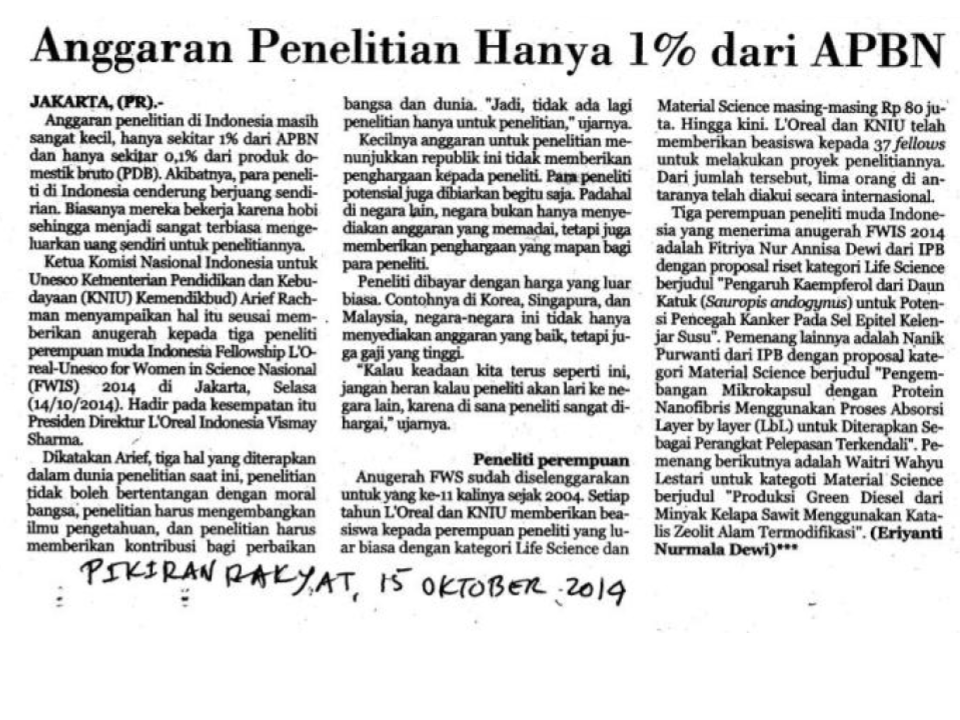
\includegraphics[width=1
	\textwidth] {pics/contoh-tulis-mentah.png} \caption{Contoh data mentah ragam tulis} 
\label{fig:contoh-tulis-mentah} \end{figure}

%-----------------------------------------------------------------------------%
\subsection{Data Jurnalistik Ragam Lisan}
%-----------------------------------------------------------------------------%
Penelitian ini memanfaatkan juga dokumentasi data jurnalistik berupa rekaman laporan berita dan wawancara dengan narasumber dengan waktu rekaman dari tahun 2013 hingga 2018. Pengumpulan data ragam lisan dilakukan bekerja sama dengan para jurnalis berbagai daerah di Indonesia yang mengunggah rekaman secara online dan video jurnalistik online yang ditranskripsi. Jumlah data ragam lisan yang terkumpul adalah 100.000 kata. Pemilahan data ragam lisan untuk dimasukkan ke dalam korpus berdasarkan kriteria sebagai berikut:

\begin{itemize}
	\item Jenis media mencakup televisi, radio, surat kabar, dan tabloid
	\item Topik mencakup politik, ekonomi, hiburan, olahraga, kebudayaan, dan teknologi
	\item Isi rekaman berupa laporan berita atau wawancara dengan narasumber
\end{itemize}

Sebelum melalui tahap berikutnya, verifikasi terhadap isi rekaman saya lakukan untuk memastikan tidak lebih dari 10\% isi rekaman yang bersifat pembacaan naskah. Hal ini menjadi perhatian penting untuk mendapatkan kualitas data korpus yang mendekati murni lisan. Data jurnalistik ragam lisan seperti pada \pic~\ref{fig:contoh-transkripsi-lisan} perlu ditranskripsi menjadi tulisan dengan metode komputasional dan diverifikasi secara manual agar dapat dianalisis dengan metode serupa seperti yang dilakukan terhadap data ragam tulis. 

\begin{itemize}
	\item Untuk melihat perbandingan dasar antara ujaran formal dengan ujaran yang lebih spontan, maka data korpus perlu diklasifikasikan menjadi data ragam tulis dan ragam lisan.
	\item Topik mencakup politik, ekonomi, hiburan, olahraga, kebudayaan, dan teknologi
	\item Isi rekaman berupa laporan berita atau wawancara dengan narasumber
\end{itemize}

\begin{figure}
	\centering 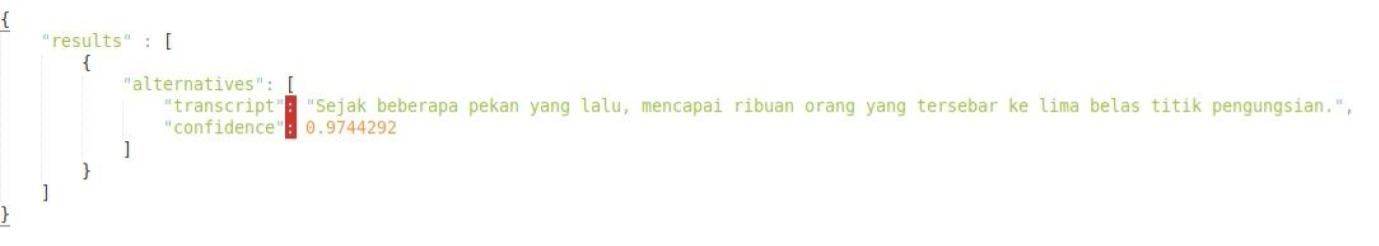
\includegraphics[width=1
	\textwidth] {pics/contoh-transkripsi-lisan.png} 
	\caption{Contoh hasil transkripsi data ragam lisan} 
	\label{fig:contoh-transkripsi-lisan} 
\end{figure}

%-----------------------------------------------------------------------------%
\section{Pengolahan Data}
%-----------------------------------------------------------------------------%
%-----------------------------------------------------------------------------%
\subsection{Klasifikasi Data}
%-----------------------------------------------------------------------------%
Berdasarkan pokok masalah yang telah dijabarkan, beberapa klasifikasi data saya lakukan untuk memperoleh analisis yang dapat menjawab pertanyaan penelitian secara tepat sasaran (Tabel \ref{tab:tabel_klasifikasi_data}).


\begin{itemize}
	\item Untuk melihat perbandingan dasar antara ujaran formal dengan ujaran yang lebih spontan, maka data korpus perlu diklasifikasikan menjadi data ragam tulis dan ragam lisan.
	\item Terkait dengan uraian permasalahan mengenai pengaruh panjang kalimat dalam penyusunan struktur ujaran yang mungkin juga mempengaruhi jarak dan arah dependensi, maka data korpus akan diklasifikasikan menjadi 3 berdasarkan panjang kalimat di bawah 10 kata, 11 hingga 20 kata, dan di atas 20 kata. Pendekatan ini menindaklanjuti temuan penelitian Oya (2011) serta Jiang dan Liu (2015) yang menggunakan klasifikasi serupa. 
	\item Sebanyak 10 kalimat yang mewakili pola terbanyak saya klasifikasikan menjadi 2 berdasarkan simpai sentralnya (central node), yaitu simpai verba dan simpai non-verba untuk analisis kualitatif guna mengeksplorasi perubahan valensi verba induk.

\end{itemize}
\begin{table}
\begin{center}
  \caption{Klasifikasi data penelitian}\label{tab:tabel_klasifikasi_data}
  \begin{tabular}{ | l | l | l | l |}
    \hline
    Ragam / Panjang kalimat & \textless 10 kata & 11 - 20 kata & \textgreater 20 kata \\ \hline
    Tulis & Tulis \textless 10 kata & Tulis 11 - 20 kata & Tulis \textgreater 20 kata  \\ \hline
    Lisan & Lisan \textless 10 kata & Lisan 11 - 20 kata & Lisan \textgreater 20 kata \\
    \hline
  \end{tabular}
\end{center}
\end{table}

%-----------------------------------------------------------------------------%
\subsection{Perangkat Pengolahan Data}
%-----------------------------------------------------------------------------%
Data jurnalistik ragam tulis yang saya terima dari hasil kerja sama dengan perusahaan media monitoring Dattabot berbentuk teks hasil pemindaian media cetak dengan menggunakan perangkat lunak Optical Character Recognition (OCR). Sedangkan, data jurnalistik ragam lisan berupa rekaman audio yang saya olah terlebih dahulu menggunakan metode komputasional dengan bantuan Google Speech API dan diverifikasi kembali secara manual. Pada tahap penguraian kalimat, saya memanfaatkan UDPipe (Straka & Strakov�, 2017), sebuah kerangka kerja yang dapat dilatih ulang untuk pengkategorian token,  penguraian lemma, dan penguraian kalimat. Penguraian kalimat dalam ranah linguistik komputasional lebih banyak ditemukan memanfaatkan teori konstituensi sebagai dasarnya sehingga menghasilkan uraian kalimat berdasarkan struktur frasanya. Penguraian kalimat ini menggunakan dasar treebank dependensi Universal Dependencies 2.0 (Nivre dkk, 2017) dengan memadukan lemma dan fitur morfologis lainnya dari MorphInd (Larasati, Kubo?, & Zeman, 2011). Analisis teks, penghitungan pola pengurangan jarak dependensi dan uji signifikansi memanfaatkan bahasa pemrograman R (versi 3.3.3) (R Core Team, 2017) dan Python (versi 3.6.3) (Python Core Team, 2017). Penelitian tesis ini juga menggunakan perangkat lunak Gephi (Bastian, Heymann, & Jacomy, 2009) untuk visualisasi data.


%-----------------------------------------------------------------------------%
\subsection{Penguraian Kalimat}
%-----------------------------------------------------------------------------%
Fitur utama dalam menguraikan tautan dependensi sintaktik dapat dilihat pada \pic~\ref{fig:tautandependensi} (Tesni�re, 1959; Hudson, 1990; Liu, 2009): tautan asimetris dan biner antara dua unit linguistik. Tautan dependensi direpresentasikan oleh panah yang mengarah dari governor atau konstituen induk ke dependent atau konstituen terikat. Kedua konstituen memiliki tautan dengan anotasi tipe dependensi di atasnya. Seluruh proses ini dilakukan dengan metode komputasional dengan bantuan UDPipe (Straka & Strakov�, 2017) dengan dasar treebank dependensi Universal Dependencies 2.0 (Nivre dkk, 2017) yang kemudian dikoreksi secara manual.

\begin{figure}
	\centering 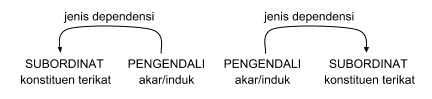
\includegraphics[width=1
	\textwidth] {pics/tautandependensi.png} \caption{Elemen-elemen dari tautan dependensi} 
\label{fig:tautandependensi} \end{figure}

Penguraian kalimat merupakan tahapan komputasional utama untuk pengolahan data penelitian sesuai dengan teori yang dijabarkan di atas. Penguraian kalimat ini mengadopsi Indonesian UD, treebank hasil konversi Universal Dependencies 2.0 (Nivre dkk, 2017) yang dikondisikan khusus untuk Bahasa Indonesia. Kata-kata di dalam kalimat memiliki tautan langsung dengan anotasi tipe dependensi di atasnya. Tipe anotasi seperti pada contoh \pic~\ref{fig:contohtulis} dan \pic~\ref{fig:contohlisan}  ini menyesuaikan dengan daftar anotasi dalam panduan dependensi milik Stanford Parser (De Marneffe & Manning, 2016 [2008]). Skema anotasi ini bersifat lintas bahasa yang awalnya dikembangkan untuk Bahasa Inggris kemudian berkembang menjadi 60 bahasa, termasuk Bahasa Indonesia. 

\begin{figure}
	\centering 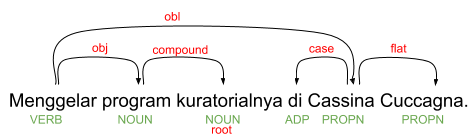
\includegraphics[width=1
	\textwidth] {pics/contohtulis.png} \caption{Contoh hasil penguraian kalimat untuk data ragam tulis} 
\label{fig:contohtulis} \end{figure}

\begin{figure}
	\centering 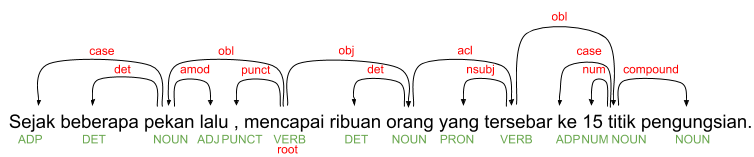
\includegraphics[width=1
	\textwidth] {pics/contohlisan.png} \caption{Contoh hasil penguraian kalimat untuk ragam lisan} 
\label{fig:contohlisan} \end{figure}

Penelitian ini mengikuti panduan dependensi milik Stanford Parser (De Marneffe & Manning, 2016 [2008]) yang mengikutsertakan tanda baca yang terlibat dalam kalimat. Penelitian ini tidak mengikutsertakan tanda baca pada akhir kalimat dalam penghitungan jarak dependensi karena tanda baca di akhir kalimat tidak memberikan pengaruh terhadap jumlah tautan dependensi yang terjadi dalam sebuah kalimat. Namun, tanda baca pada akhir kalimat tetap diperhatikan untuk analisis karena dapat menjadi indikasi perbedaan jenis kalimat maka yang mendorong perbedaan perilaku tautan dependensi yang ada. Dependensi tipe Stanford (De Marneffe & Manning, 2016 [2008]) umumnya memilih kata penuh dibandingkan dengan kata tugas sebagai induk sintaktis, kecuali untuk konstruksi kopula (tergantung kasus) dan frasa adposisi, seperti pada treebank Bahasa Indonesia dalam Universal Dependencies 2.0 (Nivre dkk, 2017). \tab~\ref{tab:tipe_anotasi} berikut berisi anotasi tipe dependensi dan deskripsi singkat berdasarkan Universal Dependencies 2.0 (Nivre dkk, 2017).

\begin{center}
\begin{small}
\begin{longtable}{| p{.20\textwidth} | p{.80\textwidth} |} 
\caption{Tipe anotasi dan deskripsi singkat berdasarkan Universal Dependencies 2.0 \citep{nivre2006maltparser}} \label{tab:tipe_anotasi}
    \hline
Anotasi & Deskripsi Tipe Anotasi \\ \hline
ROOT & Induk pohon dependensi \\ \hline
acomp & Pelengkap ajektival, termasuk pelengkap predikatif \\ \hline
adp / adpos & Adposisi yang dianalisis sebagai konstituen yang bergantung pada nomina \\ \hline
adpcomp / pcomp & Pelengkap klausal dari adposisi \\ \hline
adpmod / prep / postp & Pewatas adposisi \\ \hline
adpobj / pobj & Pelengkap nominal dari adposisi \\ \hline
advcl & Pewatas klausa adverbial \\ \hline
advmod & Pewatas adverbial \\ \hline
amod & Pewatas apposisi \\ \hline
attr & Pelengkap predikatif nominal (bergantung pada verba kopula) \\ \hline
aux & Verba bantu (bergantung pada verba induk) \\ \hline
auxpass & Verba bantu pada konstruksi pasif \\ \hline
cc & Konjungsi koordinatif (bergantung pada konjungsi) \\ \hline
ccomp & Pelengkap klausal \\ \hline
ccompmod & Pewatas kompositum (bagian kompositum yang bukan induk) \\ \hline
conj & Konjungsi \\ \hline
cop & Verba kopula \\ \hline
csubj & Subyek klausal \\ \hline
csubjpass & Subyek klausal dalam konstruksi pasif \\ \hline
dep & Konstituen terikat yang tidak terklasifikasi \\ \hline
det & Determinator \\ \hline
dobj & Obyek langsung \\ \hline
expl & Subyek (seruan) \\ \hline
infmod & Pewatas infinitif \\ \hline
iobj & Obyek tidak langsung \\ \hline
mark & Konjungsi subordinat dan ekspresi setara \\ \hline
mwe & Ekspresi multi kata, termasuk nama dengan multi kata \\ \hline
neg & Negasi \\ \hline
nmod / nommod / nommod-own / npadvmod & Pewatas nominal \\ \hline
nsubj & Subyek nominal \\ \hline
nsubjpass & Subyek nominal dalam konstruksi pasif \\ \hline
num & Numeralia \\ \hline
p / punct & Tanda baca \\ \hline
parataxis & Struktur serupa klausa yang bergantung pada klausa sebelumnya \\ \hline
partmod & Pewatas partisipel \\ \hline
poss & Pewatas posesif (atau genitif) \\ \hline
prt & Partikel verba \\ \hline
rcmod & Pewatas klausa relatif \\ \hline
rel & Pronomina atau adverbia relatif dengan fungsi yang tidak terklasifikasi \\ \hline
vmod & Pewatas verbal \\ \hline
xcomp & Pelengkap infinit serupa klausa \\ \hline
    \hline
  \end{longtable}
\end{small}
\end{center}

Kontekstualisasi treebank dependensi yang bersifat lintas bahasa dilakukan dengan melibatkan MorphInd (Larasati, Kubo?, & Zeman, 2011), sebuah pendekatan morfologis dan penguraian lemma untuk pengolahan bahasa. MorphInd memiliki aturan morfofonemik dan morfosintaktis untuk menganalisis kata-kata Bahasa Indonesia yang mengalami infleksi dan derivasi. Hasil olahan MorphInd mengintegrasikan penandaan morfologis pada sebuah kata seperti pada \pic~\ref{fig:morphind_schema}.

\begin{figure}
	\centering 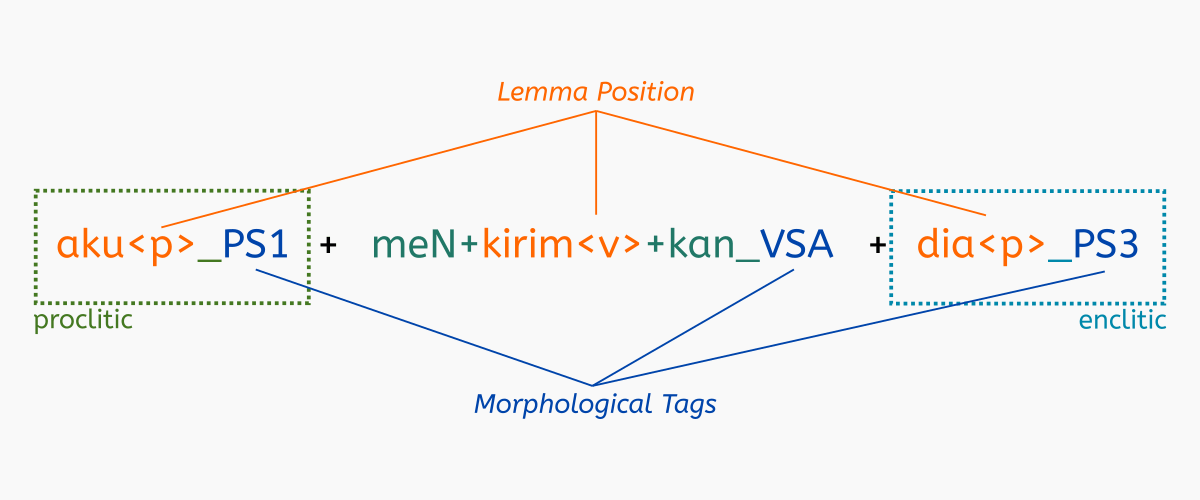
\includegraphics[width=1
	\textwidth] {pics/morphind_schema.png} \caption{Contoh hasil ekstraksi lemma dengan memanfaatkan MorphInd (Larasati, Kubo?, & Zeman, 2011) } 
\label{fig:morphind_schema} 
\end{figure}

%-----------------------------------------------------------------------------%
\section{Teknik Analsis Data}
%-----------------------------------------------------------------------------%
%-----------------------------------------------------------------------------%
\subsection{Jarak Dependensi Antarkata}
%-----------------------------------------------------------------------------%
Kalimat-kalimat di dalam korpus diperlakukan sebagai deretan kata $W1...Wi...Wn$. Jarak dependensi antara kata $Wa$ dengan kata $Wb$ dapat dihitung dari selisih $a-b$ (Liu, 2008, 2017; Futrell, 2015) sehingga kata-kata yang bersebelahan memiliki jarak dependensi sejumlah 1. Untuk memperhitungkan arah dependensi, maka apabila $a$ lebih besar dari $b$ (konstituen utama setelah konstituen terikat) akan diberi anotasi positif. Sedangkan, apabila $a$ lebih kecil dari $b$ (konstituen utama sebelum konstituen terikat) akan diberi anotasi negatif. Namun, ukuran jumlah keseluruhan dan rata-rata jarak dependensi bersifat absolut. Penelitian ini menggunakan pendekatan Jarak Dependensi atau Dependency Distance (DD) (Liu, 2007) dengan rumus penghitungan Rata-rata Jarak Dependensi atau Mean Dependency Distance (MDD) dari sebuah kalimat dengan rumus:

\noindent \begin{align}\label{eq:bola}
	\frac{1}{n-1} \displaystyle\sum_{i=1}^{n-1} |DD_i|
\end{align}

Pada rumus tersebut, $n$ adalah jumlah kata di sebuah kelimat. $DDi$ adalah jarak dependensi dengan tautan sejumlah $i$. Dalam kata lain, rata-rata jarak dependensi adalah jumlah dari nilai absolut jarak dependensi dibagi dengan jumlah tautan dependensi dalam kalimat tersebut.

\begin{figure}
	\centering 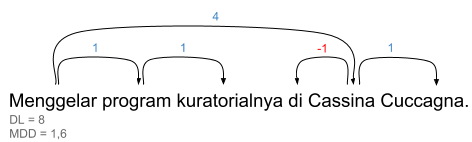
\includegraphics[width=1
	\textwidth] {pics/contohtulis_DLMDD.png} \caption{Contoh hasil olahan penghitungan jarak antarkata data ragam tulis} 
\label{fig:contohtulis_DLMDD} 
\end{figure}

\begin{figure}
	\centering 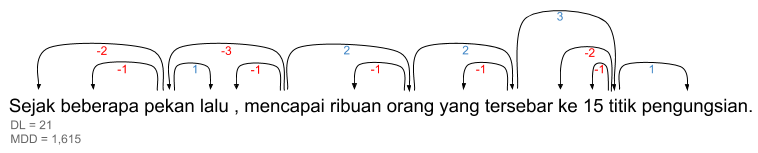
\includegraphics[width=1
	\textwidth] {pics/contohlisan_DLMDD.png} \caption{Contoh hasil olahan penghitungan jarak antarkata data ragam lisan} 
\label{fig:contohlisan_DLMDD} 
\end{figure}

Pada contoh di atas, kalimat dari ragam tulis pada \pic~\ref{fig:contohtulis_DLMDD} memiliki total jarak dependensi sejumlah 10 dan jumlah tautan dependensi sebanyak 6 sehingga nilai MDD yang didapat adalah 1.667 dengan semua arah dependensi konstituen utama sebelum konstituen terikat. Kalimat ragam tulis ini masuk ke dalam klasifikasi data ragam tulis dengan panjang kalimat kurang dari 10 kata. Sedangkan, kalimat dari ragam lisan \pic~\ref{fig:contohlisan_DLMDD} memiliki total jarak dependensi 20 dan jumlah tautan dependensi sebanyak 12 sehingga nilai MDD yang didapat adalah 1.667. Kalimat ragam lisan tersebut masuk ke dalam klasifikasi data ragam lisan dengan panjang kalimat antara 11 hingga 20 kata. Pada kedua contoh ini rata-rata jarak dependensi tidak berbeda, namun dari segi arah dependensi data ragam lisan menunjukkan karakter yang berbeda.

%-----------------------------------------------------------------------------%
\subsection{Pola Pengurangan Jarak Dependensi Antarkata}
%-----------------------------------------------------------------------------%
Berdasarkan klasifikasi data untuk penghitungan jarak dependensi antarkata melalui nilai MDD, maka saya mengadopsi beberapa pendekatan yang dilakukan oleh \cite{liu2017dependency}, \cite{futrell2015large} dan Gellman & Hill (2007). Jarak dependensi memiliki hubungan dekat dengan struktur hierarkis dan urutan linear sebuah ujaran, dan ketiga penelitian tersebut menunjukan adanya kecenderungan terhadap Pengurangan Panjang Dependensi atau Dependency Length Minimization (DLM) (Gildea & Temperley, 2010; Futrell dkk, 2015) serta Pengurangan Jarak Dependensi atau Dependency Distance Minimization (DDM) (Liu, 2009; Hudson, 2010; Ferrer-i-Cancho, 2015). Menindaklanjuti pendekatan penghitungan MDD maka penelitian ini mengacu pada hipotesis DDM dengan memanfaatkan korpus data yang telah terkumpul. Analisis pertama yang dilakukan adalah studi perbandingan MDD korpus dengan panjang kalimat terkontrol (controlled sentence length) antara korpus data hasil observasi dan korpus data kalimat acak. Dalam korpus data kalimat acak, kata-kata dalam kalimat diacak untuk menemukan nilai MDD minimum dan maksimum. Analisis ini dilakukan untuk menguji hipotesis DDM pada ujaran formal (ragam tulis) dan ujaran yang lebih spontan (ragam lisan) pada setiap golongan panjang kalimat. Uji signifikansi perlu dilakukan untuk memastikan akurasi dari pengujian hipotesis tersebut. Analisis secara kualitatif saya lakukan untuk melihat perbedaan perilaku DDM yang mungkin dipengaruhi faktor yang berbeda seperti yang dijabarkan pada uraian permasalahan.

%-----------------------------------------------------------------------------%
\subsection{Analisis Perubahan Valensi Verbal Induk}
%-----------------------------------------------------------------------------%
Pada tahap ini, saya memilih 10 kalimat dari studi perbandingan korpus dengan controlled sentence length untuk dianalisis lebih dalam secara kualitatif. Analisis ini saya lakukan untuk melihat tautan dependensi dan hubungan konstituen induk dengan konstituen terikat secara lebih dekat terutama terkait dengan perubahan valensi verbal induk. 10 kalimat dibagi menjadi 2, yaitu kalimat dengan pola dependensi yang paling banyak muncul dan kalimat dengan pola dependensi yang tidak umum dalam Bahasa Indonesia. Analisis yang dilakukan menggunakan dasar teori dependensi (Tesni�re, 1959) dan Word Grammar (Hudson, 2007, 2010) dalam menguraikan pola dependensi pada simpai sentral dengan verba sebagai konstituen induk.

Contoh kalimat ragam tulis dan lisan pada \pic~\ref{fig:contohtulis_DLMDD} dan \pic~\ref{fig:contohlisan_DLMDD}  dapat digunakan untuk mengilustrasikan analisis valensi konstituen induk. Apabila disesuaikan dengan tata bahasa yang berlaku dalam Bahasa Indonesia, kata menggelar pada kalimat Menggelar program kuratorialnya di Cassina Cuccagna dan kata mencapai pada kalimat Sejak beberapa pekan yang lalu, mencapai ribuan orang yang tersebar ke-15 titik pengungsian seharusnya sama-sama mengikat setidaknya dua actant: actant1 menggelar/mencapai actant2. Namun, kedua temuan ini sama-sama hanya mengikat satu actant yaitu actant2. 

Pertama, root dan semua konstituen terikat yang memiliki tautan dependensi langsung pada data observasi diidentifikasi kemudian diacak urutan katanya (level tautan dependensi pertama atau simpai sentral). Kemudian, konstituen terikat pada level di bawahnya yang memiliki tautan dependensi langsung diacak urutan katanya (level tautan dependensi kedua atau simpai cabang), dan seterusnya. Oleh karena itu, percobaan acak ini tidak menggunakan aturan urutan kata tertentu. Sebagai contoh, tidak ada konsistensi apakah aktor pelaku mendahului atau berada setelah verba. 

%-----------------------------------------------------------------------------%
%\section{Satu Persamaan}
%%-----------------------------------------------------------------------------%
%
%\noindent \begin{align}\label{eq:garis}
%	\cfrac{y - y_{1}}{y_{2} - y_{1}} = 
%	\cfrac{x - x_{1}}{x_{2} - x_{1}}
%\end{align}
%
%\equ~\ref{eq:garis} diatas adalah persamaan garis. 
%\equ~\ref{eq:garis} dan \ref{eq:bola} sama-sama dibuat dengan perintah \bslash
%align. 
%Perintah ini juga dapat digunakan untuk menulis lebih dari satu persamaan. 
%
%\noindent \begin{align}\label{eq:bola}
%	\underbrace{|\overline{ab}|}_{\text{pada bola $|\overline{ab}| = r$}} 
%		= \sqrt[2]{(x_{b} - x_{a})^{2} + (y_{b} - y_{a})^{2} + 
%				\vert\vert(z_{b} - z_{a})^{2}}
%\end{align}
%
%%-----------------------------------------------------------------------------%
%\section{Lebih dari Satu Persamaan}
%\label{sec:multiEqu}
%%-----------------------------------------------------------------------------%
%\noindent \begin{align}\label{eq:matriks}	
%	|\overline{a} * \overline{b}| &= |\overline{a}| |\overline{b}| \sin\theta 
%		\\[0.2cm]
%	\overline{a} * \overline{b} &=  
%		\begin{array}{| c c c |}
%			\hat{i} & x_{1} & x_{2} \\
%			\hat{j} & y_{1} & y_{2} \\
%			\hat{k} & z_{1} & z_{2} \\
%		\end{array} \nonumber \\[0.2cm]
%	&= \hat{i} \,
%		\begin{array}{ | c c | }
%			y_{1} & y_{2} \\
%			z_{1} & z_{2} \\
%		\end{array} 
%	   + \hat{j} \,
%		\begin{array}{ | c c | }
%			z_{1} & z_{2} \\
%			x_{1} & x_{2} \\
%		\end{array} 
%	   + \hat{k} \,	
%		\begin{array}{ | c c | }
%			x_{1} & x_{2} \\
%			y_{1} & y_{2} \\
%		\end{array}
%		\nonumber
%\end{align}
%
%Pada \equ~\ref{eq:matriks} dapat dilihat beberapa baris menjadi satu bagian 
%dari \equ~\ref{eq:matriks}. 
%Sedangkan dibawah ini dapat dilihat bahwa dengan cara yang sama, \equ~
%\ref{eq:gabungan1}, \ref{eq:gabungan2}, dan \ref{eq:gabungan3} memiliki nomor 
%persamaannya masing-masing. 
%
%\noindent \begin{align}\label{eq:gabungan1}	
%	\int_{a}^{b} f(x)\, dx + \int_{b}^{c} f(x) \, dx = \int_{a}^{c} f(x) \, dx
%		\\\label{eq:gabungan2}
%	\lim_{x \to \infty} \frac{f(x)}{g(x)} = 0 \hspace{1cm} 
%		\text{jika pangkat $f(x)$ $<$ pangkat $g(x)$} \\\label{eq:gabungan3}
%	a^{m^{a \, ^{n}\log b }} = b^{\frac{m}{n}}
%\end{align}
%
